\section*{Cycle 2 Experiment 12}

\section{\Large{Concurrent File Server}}

\subsection{Aim}
\large To develop concurrent file server which will provide the file requested by client if it exists. If not server sends appropriate message to the client. Server should also send its process ID (PID) to clients for display along with file or the message.

\subsection{Theory}
\textbf{Server} - A server is a software that waits for client requests and serves or processes
them accordingly.\\ \\
\textbf{Client} - A client is requester of this service. A client program request for some
resources to the server and server responds to that request.\\ \\
\textbf{Socket} - It is the endpoint of a bidirectional communication channel between a server and a client. Sockets may communicate within a process, between processes on the same machine, or between processes on different machines. For any communication with a remote program, we have to connect through a socket port.\\ \\
\textbf{FTP (File Transfer Protocol)} is a client-server protocol that may be used to transfer files between computers on the internet. The client asks for the files and the server provides them. It is a standard network protocol used for the transfer of computer files between a client and server on a computer network. FTP is built on a client-server model architecture and uses separate control and data connections between the client and the server.FTP users may authenticate themselves with a clear-text sign-in protocol, normally in the form of a username and password, but can connect anonymously if the server is configured to allow it.
\subsection{Algorithm}
\begin{verbatim}
Algorithm for the Client

1 START
2 Create the socket using the function socket()
3 Configure socket details
4 Connect the socket to server using function connect()
5 Send the name of the file to searchfor to the server
6 If found, receive the file
7 If not found, console out the appropriate message 
8 Receive the server's PID 
9 Terminate connection
10 STOP



Algorithm for the Server

1 START
2 Configure socket details
3 Bind the address struct to the socket using bind()
4 Listen to the socket
5 A new socket for the incoming connection is created using accept()
6 Reciee the name of the file to search for
7 Check for the file using access()
8 If the file is found, goto step 9, else goto step 10
9 Send the file to the client using sendfile()
10 Send the response ”NO” to the client
11 Send the PID to the client
12 STOP
\end{verbatim}

\subsection{Program \& Output}
\begin{verbatim}
//Concurrent File Server
//Client side

#include <stdio.h>
#include <fcntl.h>
#include <string.h>
#include <stdlib.h>
#include <stdbool.h>
#include <sys/stat.h>
#include <arpa/inet.h>
#include <sys/socket.h>
#include <sys/sendfile.h>

#define PORT 8080

int main()
{
    int socketServer;
    struct sockaddr_in server;
    char requestMessage[BUFSIZ], replyMessage[BUFSIZ];

    int filesize, file;
    char *data, filename[20], storageFile[20];

    socketServer = socket(AF_INET, SOCK_STREAM, 0);
    if (socketServer == -1)
    {
        perror("SOCKET NOT CREATED");
        return 1;
    }
    printf("Socket created successfully!\n");

    server.sin_addr.s_addr = inet_addr("127.0.0.1");
    server.sin_family = AF_INET;
    server.sin_port = htons(PORT);

    if (connect(socketServer, (struct sockaddr *)&server, sizeof(server)) < 0)
    {
        perror("Connection failed...");
        return 1;
    }
    printf("Connection successful!\n");

    printf("Enter the name of file to search: ");
    scanf("%s", filename);

    write(socketServer, filename, strlen(filename));
    recv(socketServer, replyMessage, 10, 0);
    int pid = atoi(replyMessage);
    printf("Process ID: %d\n", pid);
    if (pid > 0)
    {
        printf("File found!!\n");
        printf("Enter the name of the file to store data: ");
        scanf("%s", storageFile);

        recv(socketServer, &filesize, sizeof(int), 0);
        data = malloc(filesize);
        file = open(storageFile, O_CREAT | O_EXCL | O_WRONLY, 0666);
        recv(socketServer, data, filesize, 0);
        write(file, data, filesize);

        printf("File copied!\n");
        close(file);
    }
    else if (strcmp(replyMessage, "NO") == 0)
    {
        fprintf(stderr, "File not found!\n");
    }
    return 0;
}

//Server side

#include <stdio.h>
#include <fcntl.h>
#include <string.h>
#include <stdlib.h>
#include <pthread.h>
#include <stdbool.h>
#include <sys/stat.h>
#include <arpa/inet.h>
#include <sys/socket.h>
#include <sys/sendfile.h>

#define PORT 8080

void Sender(int socket, char *filename)
{
    struct stat obj;
    int file, filesize;
    stat(filename, &obj);
    file = open(filename, O_RDONLY);
    filesize = obj.st_size;

    send(socket, &filesize, sizeof(int), 0);
    sendfile(socket, file, NULL, filesize);
    printf("File sent to the client!\n");
}

void *callBack(void *socket)
{
    int socketfd = *(int *)socket;
    char serverResponse[BUFSIZ], filename[BUFSIZ];
    recv(socketfd, filename, BUFSIZ, 0);
    //If the file exists, notify the client and send it
    if (access(filename, F_OK) != -1)
    {
        snprintf(serverResponse, 10, "%d", getpid());
        write(socketfd, serverResponse, 10);
        Sender(socketfd, filename);
    }
    else
    {
        strcpy(serverResponse, "NO");
        write(socketfd, serverResponse, strlen(serverResponse));
    }
    free(socket);
}

int main(int argc, char **argv)
{
    int socketServer, socketClient, *newSocket, len = sizeof(struct sockaddr_in);
    struct sockaddr_in server, client;

    socketServer = socket(AF_INET, SOCK_STREAM, 0);
    if (socketServer == -1)
    {
        printf("SOCKET NOT CREATED");
        exit(0);
    }
    printf("Socket created successfully!\n");

    server.sin_addr.s_addr = INADDR_ANY;
    server.sin_family = AF_INET;
    server.sin_port = htons(PORT);

    if (bind(socketServer, (struct sockaddr *)&server, sizeof(server)) < 0)
    {
        printf("BIND FAILED");
        exit(0);
    }
    printf("Binding successful!\n");
    listen(socketServer, 3);
    printf("Listening for incoming connections!\n");

    while (socketClient = accept(socketServer, (struct sockaddr *)&client, 
        (socklen_t *)&len))
    {
        printf("Client connected!\n");
        pthread_t sniffer;
        newSocket = malloc(1);
        *newSocket = socketClient;
        pthread_create(&sniffer, NULL, callBack, (void *)newSocket);
        pthread_join(sniffer, NULL);
    }
    if (socketClient < 0)
    {
        printf("Accept failed!\n");
        return 1;
    }
    return 0;
}
\end{verbatim}

\subsection{Output}
\begin{figure}[h]
            \centering
            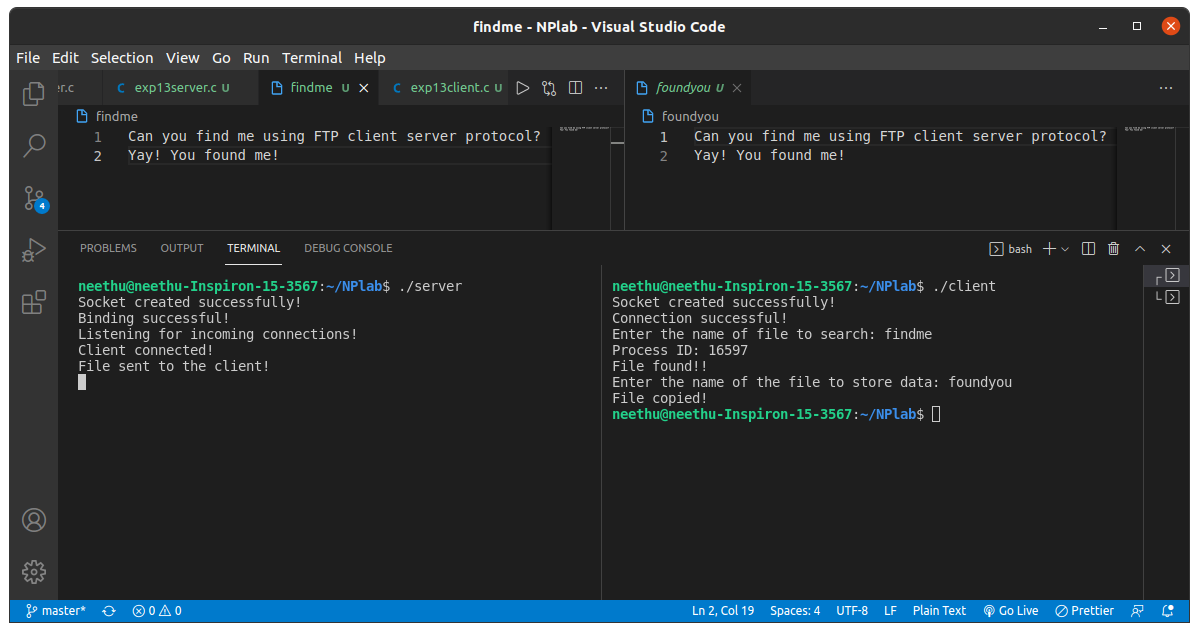
\includegraphics[scale=0.4]{img/exp12.png}
\end{figure}

\subsection{Result}
Implemented the program to develop concurrent file server which will provide the file requested by client if it exists, along with the pid, using C language in Ubuntu 20.04 with kernel and the above outputs were obtained.

